%
% $Id: $
%
%
% Compilar a .pdf con LaTeX (pdflatex)
% Es necesario instalar Beamer (paquete latex-beamer en Debian)
%

%
% Gr�ficos:
% Los gr�ficos pueden suministrarse en PNG, JPG, TIF, PDF, MPS
% Los EPS deben convertirse a PDF (usar epstopdf)
%

\documentclass{beamer}
\usetheme{GSyC}
%\usebackgroundtemplate{\includegraphics[width=\paperwidth]{format/libresoft-bg.png}}
%\usepackage[spanish]{babel}
\usepackage[latin1]{inputenc}
\usepackage{graphics}
\usepackage{amssymb} % Simbolos matematicos

\ProcessOptions

%% Metadatos del PDF.
\hypersetup{
  pdftitle={Protocolos para la Transmisi�n de Audio y V�deo por Internet},
  pdfauthor={Gregorio Robles, Jes�s M. Gonz�lez Barahona},
  pdfcreator={GSyC, Universidad Rey Juan Carlos},
  pdfproducer=PDFLaTeX,
  pdfsubject={Protocolos para la Transmisi�n de Audio y V�deo por Internet},
}
%%

\begin{document}

\title{Propiedad Intelectual - Licencias}
\subtitle{Protocolos para la Transmisi�n de Audio y V�deo en Internet}
\institute{\{grex,jgb\}@gsyc.urjc.es \\
GSyC, Universidad Rey Juan Carlos}
\author[Gregorio Robles, Jes�s M. Gonz�lez Barahona]{Gregorio Robles, Jes�s M. Gonz�lez Barahona}
\date[Nov 2014]{5 de noviembre de 2014}


\frame{
\maketitle
}


% Si el titulo o el autor se quieren acortar para los pies de p�gina
% se pueden redefinir aqu�:
%\title{Titulo corto}
%\author{Autores abreviado}


%% LICENCIA DE REDISTRIBUCION DE LAS TRANSPAS
\frame{
~
\vspace{4cm}

\begin{flushright}

\includegraphics[width=2.2cm]{figs/by-sa}

{\tiny
(cc) 2014 Gregorio Robles, Jes�s M. Gonz�lez Barahona \\
  Some rights reserved. This work licensed under Creative Commons \\
  Attribution-ShareAlike License. To view a copy of full license, see \\
\ \\
  http://creativecommons.org/licenses/by-sa/3.0/ or write to \\
  Creative Commons, 559 Nathan Abbott Way, Stanford, \\
  California 94305, USA. \\
\ 
}
\end{flushright}
}
%%

%-----------------------    ---------------------------------

\begin{frame}
\frametitle{�Qu� es la Propiedad Intelectual? �Y las licencias?}

\begin{itemize}
   \item La PI es la que regula qu� se puede hacer con obras de car�cter intelectual
   \item Se divide en dos partes
   \begin{itemize}
      \item Derechos morales (autor�a, etc.). La mayor�a irrenunciables y eternos
      \item Derechos de explotaci�n (difusi�n, representaci�n, copia...). Limitados en el tiempo.
   \end{itemize}
   \item Por defecto, el autor no te cede ning�n derecho
   \item ... en la licencia vienen las condiciones de uso
\end{itemize}

\end{frame}


%-----------------------    ---------------------------------

\begin{frame}
\frametitle{Software libre}

\begin{enumerate}
  \setcounter{enumi}{-1}
   \item Permite su uso, con cualquier prop�sito
   \item Permite su estudio y su modificaci�n
   \item Permite distribuir copias
   \item Permite mejorar y hacer p�blicas las mejoras.
\end{enumerate}

\begin{itemize}
  \item Hay muchas licencias de software libre: las m�s conocidas son la GNU GPL, la de Apache o las BSDs
  \item Hay licencias para otros contenidos (m�sica, escritos...) como las Creative Commons
  \item El software libre no tiene por qu� ser gratis.
  \item En GitHub, al iniciar un proyecto te pregunta por la licencia
\end{itemize}

\end{frame}

%-----------------------    ---------------------------------

\begin{frame}
\frametitle{Richard Stallman}

\begin{center}
  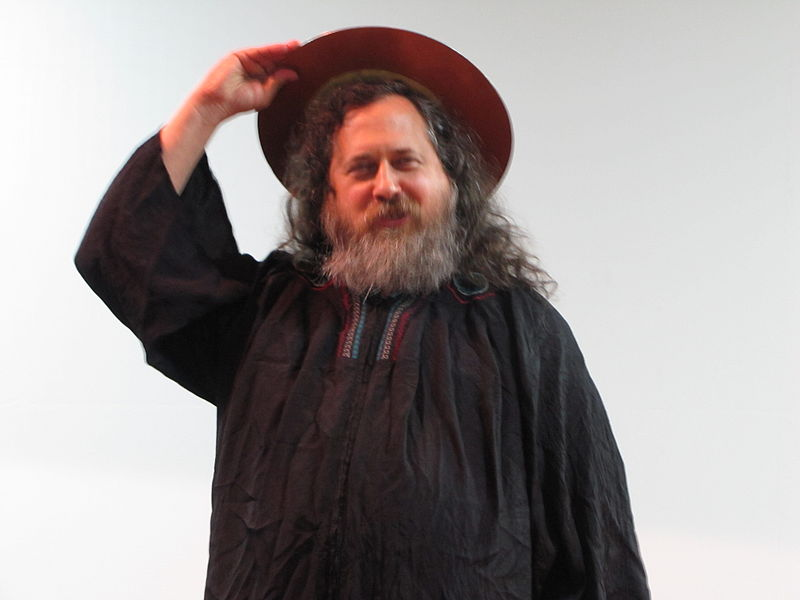
\includegraphics[width=10cm]{figs/stallman.jpg}
\end{center}


\begin{flushright}
{\tiny
Source: http://lunduke.com/wp-content/uploads/2012/03/RMS\_iGNUcius\_techfest\_iitb.jpeg
}
\end{flushright}

\end{frame}


\frame{
\maketitle
}

\end{document}
